\documentclass{ximera}

\title{Function Review Activity}
\author{MATH 425: Calculus I}

\begin{document}
\begin{abstract}
    Working with the peers in your group, solve the following problems. Make sure to show and justify all your work. Make sure everyone in the group understands the solution and participates. Be prepared to report your answers to the whole class. 
\end{abstract}
\maketitle


\begin{exercise}

 In this problem, let $x$ denote the length of the base of a rectangle. Suppose the height of the rectangle is always half the length of its base.
    \begin{enumerate}
        \item Draw a labeled sketch of the rectangle.
        \begin{image}
         \includegraphics{funcreview1A.png}
        \end{image}
        \item Let $A(x)$ be a function that gives the area of the rectangle whose base has length $x$. Find a formula for $A(x)$ as a function of $x$.\\
        \textcolor{blue}{$A(x)=(\frac{1}{2}x)x=\frac12 x^2$}
        \item What is the domain of the function $A(x)$? Explain your answer.\\
        \textcolor{blue}{Only positive values of $x$ make sense, as $x$ is representing a length. Domain: all real positive numbers, or $(0,\infty)$.}
        \item Let $P(x)$ be a function that gives the perimeter of the rectangle whose base has length $x$. Find a formula for $P(x)$ as a function of $x$.\\
        \textcolor{blue}{$P(x)=2x+2(\frac12x)=2x+x=3x$}
       % Using the work you did on your homework, 
       \item Write the area of the rectangle, $A(x)$, in terms of the perimeter $P(x)$.\\
       \textcolor{blue}{We can solve $P(x)=3x$ for $x$: $x=\frac{P(x)}{3}$\\
       Sub this value into $A(x)=A(\frac{P(x)}{3})=\frac12(\frac{P(x)}{3})^2=\frac{(P(x))^2}{18}} 
    \end{enumerate}
\end{exercise}

\begin{exercise}
   Determine the domain of the function $g(x)=\frac{\sqrt{x-1}}{x^2-9}$.\\
   \textcolor{blue}{The domain of a rational function is all numbers where the denominator is not 0, so we set the denominator to 0 and exclude these values.\\
   $x^2-9=0$\\
   $(x-3)(x+3)=0$\\
   $x=3,-3$\\
   We also have to take into account that we can not put a negative value into the square root.\\
   $x-1\geq 0$\\
   $x\geq 1$\\
   Taking these together we get all real numbers greater than 1, except $x=3$, or $[1,3)\cup(3,\infty)$.}
\end{exercise}

\begin{exercise}
     Suppose \[ f(x)=\begin{cases} 
     3x-2 & x< 0 \\
      x^2+1 & 0< x\leq 4 \\
      0 &  4< x 
   \end{cases}
\]
   \begin{enumerate}
    \item Evaluate $f(-2)$, $f(0)$, $f(3)$ and $f(5)$.\\
    \textcolor{blue}{\[f(-2)=3(-2)-2=-6-2=-8\]
    \[f(3)=3^2+1=10\]
    \[f(5)=0\]
    $f(0)$ does not exist, as the function is not defined at $x=0$.}
    \item Sketch a graph of the function. 
    \begin{image}
      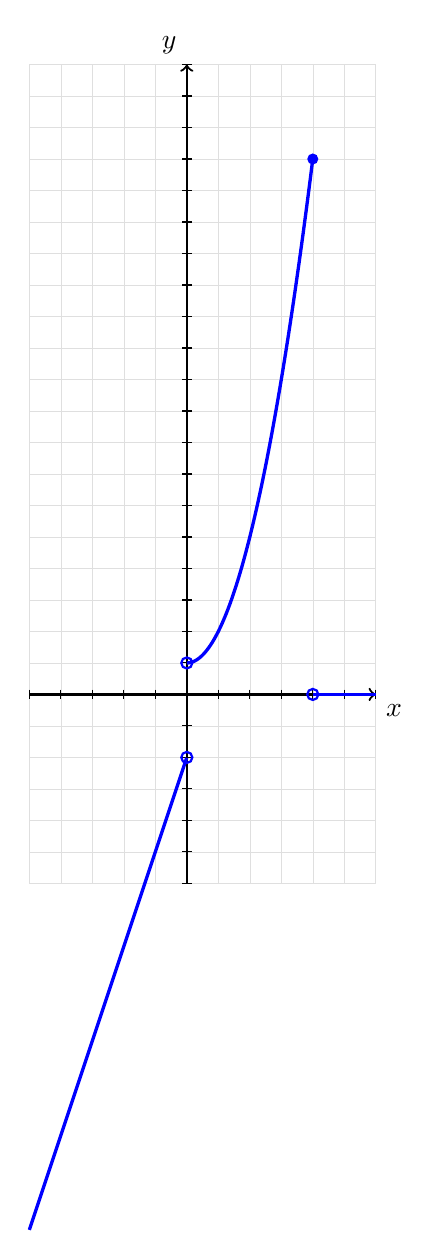
\begin{tikzpicture}[scale=0.4]
  \def\xmin{-5}
  \def\xmax{6}
  \def\ymin{-6}
  \def\ymax{20}
  \def\samples{300}
  \def\opensz{5pt}
  \def\closesz{5pt}

  % Grid (optional)
  \draw[step=1, very thin, gray!25] (\xmin,\ymin) grid (\xmax,\ymax);

  % Axes
  \draw[->, thick] (\xmin,0) -- (\xmax,0) node[below right] {$x$};
  \draw[->, thick] (0,\ymin) -- (0,\ymax) node[above left] {$y$};

  % Ticks (optional)
  \foreach \x in {\xmin,...,\xmax}{
    \draw (\x,0.15) -- (\x,-0.15);
  }
  \foreach \y in {\ymin,...,\ymax}{
    \draw (0.15,\y) -- (-0.15,\y);
  }

  % y = 3x - 2 for x < 0
  \draw[very thick, blue, samples=\samples, domain=\xmin:-0.001, smooth, variable=\x]
    plot ({\x},{3*\x - 2});
  \draw[blue, line width=0.8pt] (0,-2) circle (\opensz); % open at (0,-2)

  % y = x^2 + 1 for 0 < x <= 4
  \draw[very thick, blue, samples=\samples, domain=0.001:4, smooth, variable=\x]
    plot ({\x},{\x*\x + 1});
  \draw[blue, line width=0.8pt] (0,1) circle (\opensz);   % open at (0,1)
  \fill[blue] (4,17) circle (\closesz);                   % closed at (4,17)

  % y = 0 for x > 4
  \draw[very thick, blue] (4.01,0) -- (\xmax,0);
  \draw[blue, line width=0.8pt] (4,0) circle (\opensz);  % open at (4,0)
\end{tikzpicture}
    \end{image}
   \end{enumerate}
 
\end{exercise}

\begin{exercise}
   Consider the following functions.  Classify the functions in the following ways, and be prepared to defend your answers. \\
    $f(x)=4^x$\\
    $g(x)=x^6$\\
    $h(x)=\frac{1+2x}{1+\sqrt{x}}$\\
    $F(t)=1-2.1t+3t^2$\\
    $G(t)=\log_2(t)$\\
    $H(t)=\sqrt[3]{t}$\\
    $P(q)=\frac{2q^3}{1-q^3}$\\
    $R(m)=\sin(m)$\\
    $C(z)=z$
  \begin{enumerate}
      \item Are any of these functions classified as linear functions?  Which one(s)?\\
      \textcolor{blue}{$C(z)$}
      \item Are any of these functions classified as polynomial functions?  Which one(s)?\\
      \textcolor{blue}{$F(t)$, $g(x)$, $C(z)$}
      \item Are any of these functions classified as power functions functions?  Which one(s)?\\
      \textcolor{blue}{$g(x)$, $C(z)$, $H(t)$}
      \item Are any of these functions classified as rational functions functions?  Which one(s)?\\
      \textcolor{blue}{$P(q)$}
      \item Are any of these functions classified as algebraic functions?  Which one(s)?\\
      \textcolor{blue}{$F(t)$, $P(q)$, $g(x)$, $h(x)$, $H(t)$, $C(z)$}
  \end{enumerate}
\end{exercise}

\end{document}